\chapter{Analisi dei requisiti}
\label{cap:analisi-requisiti}

In questo capitolo vengono analizzati tutti i requisiti individuati, come ad esempio apertura ticket, chiusura ecc..\\
Lo scopo è definire con chiarezza la funzione che svolge ogni requisito all'interno dell'applicazione, andando  ad assegnare a questi un'etichetta che li identifica in base alla  loro natura.

\section{Casi d'uso}

Per lo studio dei casi di utilizzo del prodotto sono stati creati dei diagrammi.
I diagrammi dei casi d'uso (in inglese \emph{Use Case Diagram}) sono diagrammi di tipo \gls{uml} dedicati alla descrizione delle funzioni o servizi offerti da un sistema, così come sono percepiti e utilizzati dagli attori che interagiscono col sistema stesso.
Essendo il progetto finalizzato alla creazione di un tool per l'automazione di un processo, le interazioni da parte dell'utilizzatore devono essere ovviamente ridotte allo stretto necessario. Per questo motivo i diagrammi d'uso risultano semplici e in numero ridotto.

\subsection{Attori}


\begin{figure}[H]
    \centering 
    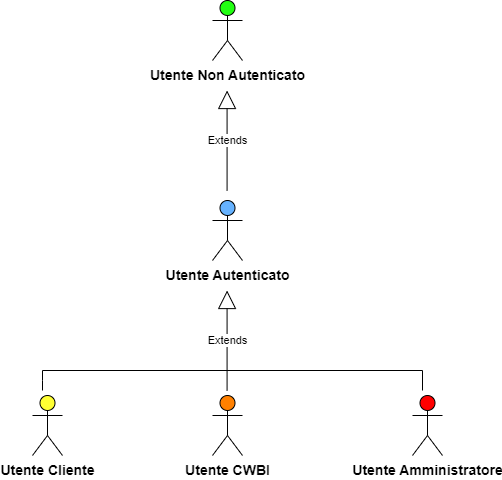
\includegraphics[width=0.9\columnwidth]{usecase/utenti-primari} 
    \caption{Gerarchia degli attori}
\end{figure}

\\
\textbf{Utente Non Autenticato}: utente che ancora non ha effettuato l'accesso alla webapp. 
\\
\textbf{Utente Autenticato}: utente che ha effetuato l'accesso.  
\\ 
\textbf{Utente Cliente}: utente autenticato con permessi di livello Cliente. Rappresenta i clienti esterni all'azienda. 
\\ 
\textbf{Utente CWBI}: utente autenticato con permessi di livello CWBI. Rappresenta i dipendenti dell'azienda CWBI. 
\\
\textbf{Utente Amministratore}: utente autenticato con permessi Amministratore. Rappresenta uno o più dipendenti CWBI che hanno la funzione di amministrare la webapp e i contenuti.  \\


\subsection{Elenco}
\subsubsection{UC01 - Autenticazione}

\begin{figure}[H]
    \centering 
    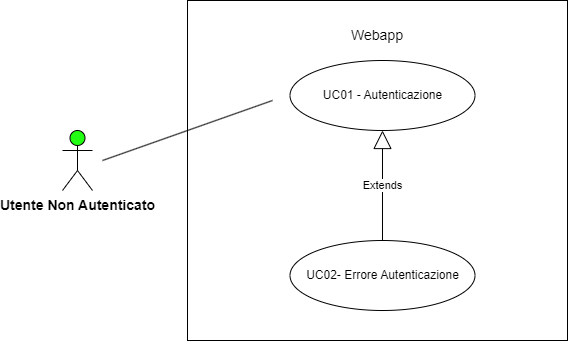
\includegraphics[width=0.9\columnwidth]{usecase/UC01}
    \caption{UC01}
\end{figure}

            \begin{table}[H]
                \centering
                \renewcommand{\arraystretch}{1.8}
                \renewcommand\tabularxcolumn[1]{m{#1}}
                \begin{tabularx}{0.9\textwidth} {
                    >{\hsize=.8\hsize\linewidth=\hsize}X
                    >{\hsize=1.2\hsize\linewidth=\hsize}X}
                    \hline
                    \textbf{Attore primario} & Utente non autenticato \\
                    \hline
                    \textbf{Precondizioni} & L'utente non è autenticato. \\
                    \hline
                    \textbf{Postcondizioni} & L'utente è autenticato. \\
                    \hline
                    \textbf{Scenario principale} & L'utente accede alla webapp \\
                    \hline
                    \textbf{Estensioni} & Se l'accesso non va a buon fine, si verifica \hyperref[UC02]{UC02}. \\
                    \hline
                \end{tabularx}
                \caption{UC01}
            \end{table}

\subsubsection{UC02 - Errore Autenticazione}

                    \begin{table}[H]
                    \centering
                    \renewcommand{\arraystretch}{1.8}
                    \renewcommand\tabularxcolumn[1]{m{#1}}
                    \begin{tabularx}{0.9\textwidth} {
                        >{\hsize=.8\hsize\linewidth=\hsize}X
                        >{\hsize=1.2\hsize\linewidth=\hsize}X}
                        \hline
                        \textbf{Attore primario} & Utente non autenticato \\
                        \hline
                        \textbf{Precondizioni} & L'utente sta tentando di autenticarsi. \\
                        \hline
                        \textbf{Postcondizioni} & L'operazione fallisce. \\
                        \hline
                        \textbf{Scenario principale} &
                            \begin{enumerate}
                                \item Si verificano problemi con l'accesso alla webapp;
                                \item Viene mostrato un errore che informa l'utente del fallimento dell'operazione.
                            \end{enumerate} \\
                        \hline
                    \end{tabularx}
                    \caption{UC02}
                \end{table}

\section{Tracciamento dei requisiti}

Da un'attenta analisi dei requisiti e degli use case effettuata sul progetto è stata stilata la tabella che traccia i requisiti in rapporto agli use case.\\
Il requisito è così descritto:
    \begin{itemize}
    \setlength\itemsep{1em}

        \item \textbf{codice identificativo}: ogni codice 				identificativo è univoco e definito seguendo lo 					standard di codifica \textbf{R[Importanza][Tipologia]				[Codice]}  il significato delle cui voci è:
        \begin{itemize}
        \setlength\itemsep{1em}

            \item \textbf{Importanza}:
            \begin{center}
                
                \renewcommand{\arraystretch}{1.8}
                \renewcommand\tabularxcolumn[1]{m{#1}}
                \begin{tabularx}{0.85\textwidth} {
                    >{\hsize=0.1\hsize\linewidth=\hsize}X
                    >{\hsize=1.9\hsize\linewidth=\hsize}X
                }
                    \hline
                    \textbf{1} & Requisito obbligatorio: 								irrinunciabile per l'azienda e i clienti \\
                    \hline
                    \textbf{2} & Requisito desiderabile: non 							strettamente necessario ma  a valore 							aggiunto riconoscibile. \\
                    \hline
                    \textbf{3} &  Requisito opzionale: 								relativamente utile oppure contrattabile 							più avanti nel progetto. \\
                    \hline
                \end{tabularx}
                \smallskip
            \end{center}
			
            \item \textbf{Tipologia}:
            \begin{center}
                
                \renewcommand{\arraystretch}{1.5}
                \begin{tabular}{m{2em} m{10em}}
                    \hline
                    \textbf{F} & Funzionale \\
                    \hline
                    \textbf{P} & Prestazionale \\
                    \hline
                    \textbf{Q} & Qualitativo \\
                    \hline
                    \textbf{V} &  Vincolo \\
                    \hline
                \end{tabular}
                \smallskip
            \end{center}
            
            \item \textbf{Codice}: identificatore univoco del 				requisito in forma gerarchica.
        \end{itemize}

		
        \item \textbf{classificazione}: viene riportata 						l'importanza del requisito per facilitare la 						lettura;
        \item \textbf{descrizione};
        \item \textbf{fonte}: origine del requisito.
    \end{itemize}

\newpage

\subsection{Requisiti funzionali}
    
\begin{table}[!h]
\caption{Tabella del tracciamento dei requisiti funzionali}
{\renewcommand{\arraystretch}{2}
\label{tab:requisiti-funzionali}
\begin{tabularx}{\textwidth}{PXl}
\hline\hline
\textbf{Requisito} & \textbf{Descrizione}\\
\hline

R1F1 & L'utente ha la possibilità di effetuare il login\\
\hline
R1F2 & L'utente con permesso Cliente ha la possibilità di poter accedere al modulo Ticket\\
\hline
R1F3 & L'utente con permesso CWBI ha la possibilità di poter accedere al modulo Ticket\\
\hline
R1F4	 & L'utente amministratore ha la possibilità di poter accedere ai vari moduli\\
\hline
R1F5 & L'utente amministratore può registrare un nuovo utente specificandone i permessi\\
\hline
R1F6 & L'utente loggato, accedendo al modulo ticket, può visualizzare la pagina di Home\\
\hline
R1F7 & L'utente loggato, accedendo al modulo ticket, può visualizzare la pagina di Menu\\
\hline
R1F8 & L'utente loggato può visualizzare i ticket aperti da lui\\
\hline
R1F9 & L'utente loggato può visualizzare i ticket presi in carico\\
\hline
R1F10 & L'utente loggato può visualizzare gli ultimi 10 ticket aperti\\
\hline

R1F11 & L'utente loggato può creare un nuovo ticket\\
\hline
R1F11.1 & L'utente loggato, quando crea un nuovo ticket, deve selezionare l'azienda di riferimento\\
\hline
R1F11.2 & L'utente loggato, deve selezionare il progetto su cui aprire il ticket\\
\hline
R1F11.3 & L'utente loggato deve inserire il titolo del ticket\\
\hline
R1F11.4 & L'utente loggato può inserire una descrizione del ticket\\
\hline
R1F11.5 & L'utente loggato deve selezionare l'ambiente su cui aprire il ticket\\
\hline
R1F11.6 & L'utente loggato deve selezionare la priorità del ticket\\
\hline

\end{tabularx}
}
\end{table}

\begin{table}[H]
{\renewcommand{\arraystretch}{2}%}
\begin{tabularx}{\textwidth}{PXl}
\hline\hline
\textbf{Requisito} & \textbf{Descrizione}\\

\hline
R1F11.7 & L'utente loggato deve selezionare lo stato del ticket\\
\hline
R1F11.8 & L'utente loggato può inserire la data di scadenza entro il quale il ticket deve essere completato\\
\hline
R1F11.9 & L'utente loggato può inserire un allegato\\
\hline
R1F12 & Il modulo visualizza la pagina di selezione dell' azienda \\
\hline
R1F12.1 & Il modulo visualizza solo e soltanto la lista delle aziende a cui è collegato l'utente loggato \\
\hline
R1F13 & Il modulo visualizza la pagina di creazione del ticket\\
\hline
R1F13.1 & visualizza solo e soltanto i progetti collegati all'azienda selezionata\\
\hline
R1F13.2 & Il modulo fornisce 3 ambienti su cui aprire il ticket: SVIL, PROD, TEST\\
\hline
R1F13.3 & Il modulo fornisce 4 gradi di priorità (1,2,3,4)\\
\hline
R1F13.4 & Il modulo fornisce 2 stati del ticket: APERTO - CHIUSO\\
\hline
R1F13.5 & Il modulo fornisce di poter allegare file di tipo: pdf/txt\\
\hline
R1F13.6 & Il modulo fornisce la possibilità di personalizzare la descrizione del ticket\\
\hline
R1F13.7 & Il modulo fornisce di annullare la creazione di un nuovo ticket\\
\hline
R1F14 & L'utente loggato può modificare un ticket\\
\hline
R1F14.1 & L'utente loggato, in fase di modifica, deve selezionare l'utente assegnatario\\
\hline
R1F15 & L'utente loggato può eliminare un ticket\\
\hline
R1F16 & L'utente loggato può visualizzare il dettaglio del ticket\\
\hline
R1F16.1 & Il modulo visulizza il titolo del ticket\\
\hline
R1F16.2 & Il modulo visualizza l'id del ticket\\
\hline
R1F16.3 & Il modulo visualizza l'etichetta stato del ticket\\
\hline
R1F16.4 & Il modulo visualizza l'etichetta priorità del ticket\\
\hline


\end{tabularx}
}
\end{table}

\begin{table}[H]
{\renewcommand{\arraystretch}{2}
\begin{tabularx}{\textwidth}{PXl}
\hline\hline
\textbf{Requisito} & \textbf{Descrizione}\\
\hline

R1F16.5 & Il modulo visualizza l'etichetta ambiente del ticket\\
\hline
R1F16.6 & Il modulo visualizza la descrizione estesa del ticket\\
\hline
R1F16.7 & Il modulo visualizza l'azienda del ticket\\
\hline
R1F16.8 & Il modulo visualizza l'assegnatario del ticket\\
\hline
R1F16.9 & Il modulo visualizza la descrizione del ticket\\
\hline
R1F16.10 & Il modulo visualizza l'assegnatario del ticket\\
\hline
R1F17 & L'utente loggato può scaricare il file allegato al ticket\\
\hline
R1F18 & L'utente loggato può cambiare lo stato del ticket dal dettaglio\\
\hline
R1F19 & L'utente può visualizzare la lista dei commenti del ticket\\
\hline
R1F19.1 & L'utente loggato può scaricare il file allegato al singolo commento\\
\hline
R1F20 & L'utente loggato può creare un nuovo commento per un ticket\\
\hline
R1F21 & L'utente loggato può modificare un commento\\
\hline
R1F22 & L'utente loggato può eliminare un commento\\
\hline
R1F23 & L'utente loggato può allegare un file al commento\\
\hline
R1F24 & L'utente loggato può visualizzare la pagina di ricerca\\
\hline

R1F25 & L''utente loggato può ricercare i ticket\\
\hline
R1F25.1 & L'utente loggato può ricercare i ticket per identificativo\\
\hline
R1F25.2 & L'utente loggato può ricercare i ticket per azienda\\
\hline
R1F25.3 & L'utente loggato può ricercare i ticket per titolo\\
\hline
R1F25.4 & L'utente loggato può ricercare i ticket per stato\\
\hline
R1F25.5 & L'utente loggato può ricercare i ticket per priorità\\
\hline
R1F25.6 & L'utente loggato può ricercare i ticket per utente assegnato\\
\hline
R1F25.7 & L'utente loggato può ricercare i ticket per ambiente\\
\hline
\end{tabularx}
}
\end{table}

\pagebreak

\begin{table}[H]
{\renewcommand{\arraystretch}{2}
\begin{tabularx}{\textwidth}{PXl}
\hline\hline
\textbf{Requisito} & \textbf{Descrizione}\\
\hline

R1F26 & Il modulo, visualizza i bottoni di modifica su ogni riga, solo se il ticket è stato aperto dall'utente attualmente loggato \\
\hline
R1F26.1& Il modulo, per ogni riga, fornisce il bottone di dettaglio del ticket \\
\hline
R1F26.2 & Il modulo, per ogni riga, fornisce il bottone di modifica del ticket \\
\hline
R1F26.3 & Il modulo, per ogni riga, fornisce il bottone di elimina del ticket \\
\hline
R1F27 & Il modulo permette si effettuare il salvataggio del ticket\\
\hline
R1F28 & Il modulo visualizza un errore in caso il salvataggio non vada a buon fine \\
\hline
R2F28.1 & Il modulo visualizza un errore in caso il titolo sia vuoto\\
\hline
R2F28.2 & Il modulo visualizza un errore in caso la data di scadenza sia vuota\\
\hline
R2F39 & Il modulo visualizza un avviso in caso non ci siano ticket da visualizzare\\
\hline
R2F30 & Il modulo visualizza un avviso dopo l'eliminazione di un ticket\\
\hline

\end{tabularx}
}
\end{table}

\bigskip

\subsection{Requisiti di vincolo}

\begin{table}[!h]
{\renewcommand{\arraystretch}{2}
\caption{Tabella del tracciamento dei requisiti di vincolo}
\label{tab:requisiti-vincolo}
\begin{tabularx}{\textwidth}{PXl}
\hline\hline
\textbf{Requisito} & \textbf{Descrizione} \\
\hline
R1V1 & Il modulo deve limitare la modifica di un ticket\\
\hline
R1V1.1 & Il modulo permette la modifica del ticket all'utente che lo ha aperto\\
\hline
R1V1.2 & Il modulo permette la modifica del ticket all'utente amministratore\\
\hline
R1V2 & Il modulo deve limitare l'eliminazione di un ticket\\
\hline
R1V2.1 & Il modulo permette l'eliminazione del ticket all'utente che lo ha aperto\\
\hline
R1V2.2 & Il modulo permette l'eliminazione del ticket all'utente amministratore\\
\hline

R1V3 & Il modulo deve limitare la modifica di un commento\\
\hline

\end{tabularx}
}
\end{table}


\begin{table}[H]
{\renewcommand{\arraystretch}{2}
\caption{Tabella del tracciamento dei requisiti di vincolo}
\label{tab:requisiti-vincolo}
\begin{tabularx}{\textwidth}{PXl}
\hline\hline
\textbf{Requisito} & \textbf{Descrizione} \\
\hline
R1V3.1 & Il modulo permette la modifica del commento all'utente che lo ha aperto\\
\hline
R1V3.2 & Il modulo permette la modifica del commento all'utente amministratore\\
\hline
R1V4 & Il modulo deve limitare l'eliminazione di un commento\\
\hline
R1V4.1 & Il modulo permette l'eliminazione del commento all'utente che lo ha aperto\\
\hline
R1V4.2 & Il modulo permette l'eliminazione del commento all'utente amministratore\\
\hline
R1V5 & Il modulo deve essere sviluppato in Java\\
\hline
R1V6 & Il modulo integra classi preesistenti in altri moduli\\
\hline
R1V7 & Il modulo deve essere sviluppato secondo l'architettura dell'azienda\\
\hline
R1V8 & Devono essere utilizzati i framework previsti dall'azienda per lo sviluppo delle applicazioni aziendali\\
\hline

\end{tabularx}
}
\end{table}


